\documentclass[10 pt]{article}

\usepackage[utf8x]{inputenc}
\usepackage{dsfont}
\usepackage{amsthm}
\usepackage{amsfonts}
\usepackage{amssymb}
\usepackage{tensor}
\usepackage{mathtools}
\usepackage[T1]{fontenc}
%\usepackage[spanish]{babel}
\usepackage[cm]{fullpage}
\usepackage{graphicx}
\usepackage{float}
\usepackage{bm}
\usepackage{setspace}
\usepackage{enumitem}
\usepackage{mdwlist}
\usepackage{parskip}
\usepackage{listings}
\usepackage{color}
%\usepackage{epstopdf}
\usepackage{tikz,datatool}
\usepackage{hyperref}

\newcommand{\HRule}{\rule{\linewidth}{0.5mm}}

\AtBeginDocument{
  \let\myThePage\thepage
  \renewcommand{\thepage}{\oldstylenums{\myThePage}}
}

\newcommand{\gra}{$^\text{o}$}
\newcommand{\dif}{\text{d}}
\newcommand{\avg}[1]{\left\langle #1 \right\rangle}
\newcommand{\ket}[1]{\left| #1 \right\rangle}
\newcommand{\bra}[1]{\left\langle #1 \right|}
\newcommand{\bket}[2]{\left\langle #1 \middle| #2 \right\rangle}
\newcommand{\der}[2]{\frac{\text{d} #1}{\text{d} #2}}
\newcommand{\prt}[2]{\frac{\partial #1}{\partial #2}}
\newcommand{\dert}[3]{\frac{\text{d}^#3 #1}{\text{d} #2^#3}}
\newcommand{\prtt}[3]{\frac{\partial^#3 #1}{\partial #2^#3}}
\newcommand{\dl}{\mathcal{L}}
\newcommand{\dha}{\mathcal{H}}
\newcommand{\vol}{\text{vol}}
\renewcommand{\vec}[1]{\pmb{#1}}

\newenvironment{algo}[1]
{  \begin{center}
   \mbox{
       \begin{minipage}{\textwidth}
           \begin{tabbing}
           \settabs
            #1
           \end{tabbing}
        \end{minipage}
    }
    \end{center}
}{}
\newcommand{\settabs}{mmm\=mmm\=mmm\=mmm\=mmm\=mmm\=\kill}

\DeclarePairedDelimiter\ceil{\lceil}{\rceil}
\DeclarePairedDelimiter\floor{\lfloor}{\rfloor}

\definecolor{mygray}{rgb}{0.4,0.4,0.4}
\definecolor{mygreen}{rgb}{0,0.5,0.25}
\definecolor{myorange}{rgb}{1.0,0.4,0}

\definecolor{clock0}{cmyk}{1,0,0,0}
\definecolor{clock1}{cmyk}{1,1,0,0}
\definecolor{clock2}{cmyk}{0,1,0,0}
\definecolor{clock3}{cmyk}{0,1,1,0}
\definecolor{clock4}{cmyk}{1,0,1,0}
\definecolor{clock5}{cmyk}{1,1,1,0}
\definecolor{clock6}{cmyk}{0,0,1,0}
\definecolor{clock7}{cmyk}{0,0,0,0.1}

\begin{document}

\lstset{
language=C++,
basicstyle=\ttfamily\color{black},
commentstyle=\color{mygray}\ttfamily,
frame=single,
numbers=left,
numbersep=5pt,
numberstyle=\tiny\color{mygray}\ttfamily,
keywordstyle=\color{mygreen}\ttfamily,
showspaces=false,
showstringspaces=false,
stringstyle=\color{myorange}\ttfamily,
tabsize=2,
emph={double,uint8_t,uint16_t,uint32_t,uint64_t,int8_t,int16_t,int32_t,int64_t},
emphstyle={\color{blue}\ttfamily}
}

\begin{center}
  \Large \textsc{Week 8: Ornstein-Zernike solver}
\end{center}

\begin{center}
  \large \textsc{Francisco García Flórez}
\end{center}

\section{Results}

Using the Ornstein-Zernike solver with Percus-Yevick approximation, with a tolerance of $10^{-9}$ and 4096 grid points for the numerical Fourier transform, we found the following results.

\begin{figure}[H]
  \begin{center}
    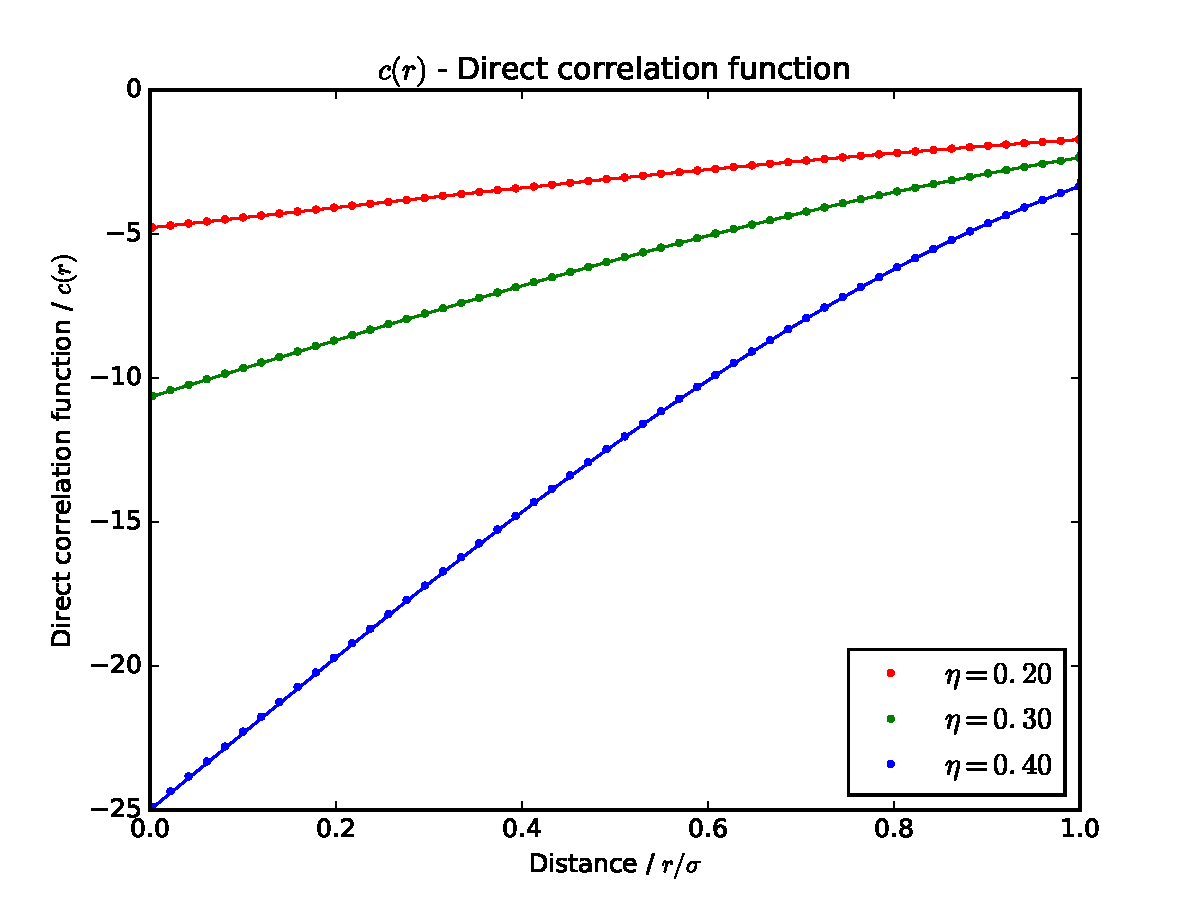
\includegraphics[width=0.7\textwidth]{{../graphs/ozsolver-c}.pdf}
  \end{center}
  \caption{Plot of the direct correlation function, $c(r)$, for several values of $\eta$. Points are values computed using the OZ solver, and lines are theoretical values.}
\end{figure}

\begin{figure}[H]
  \begin{center}
    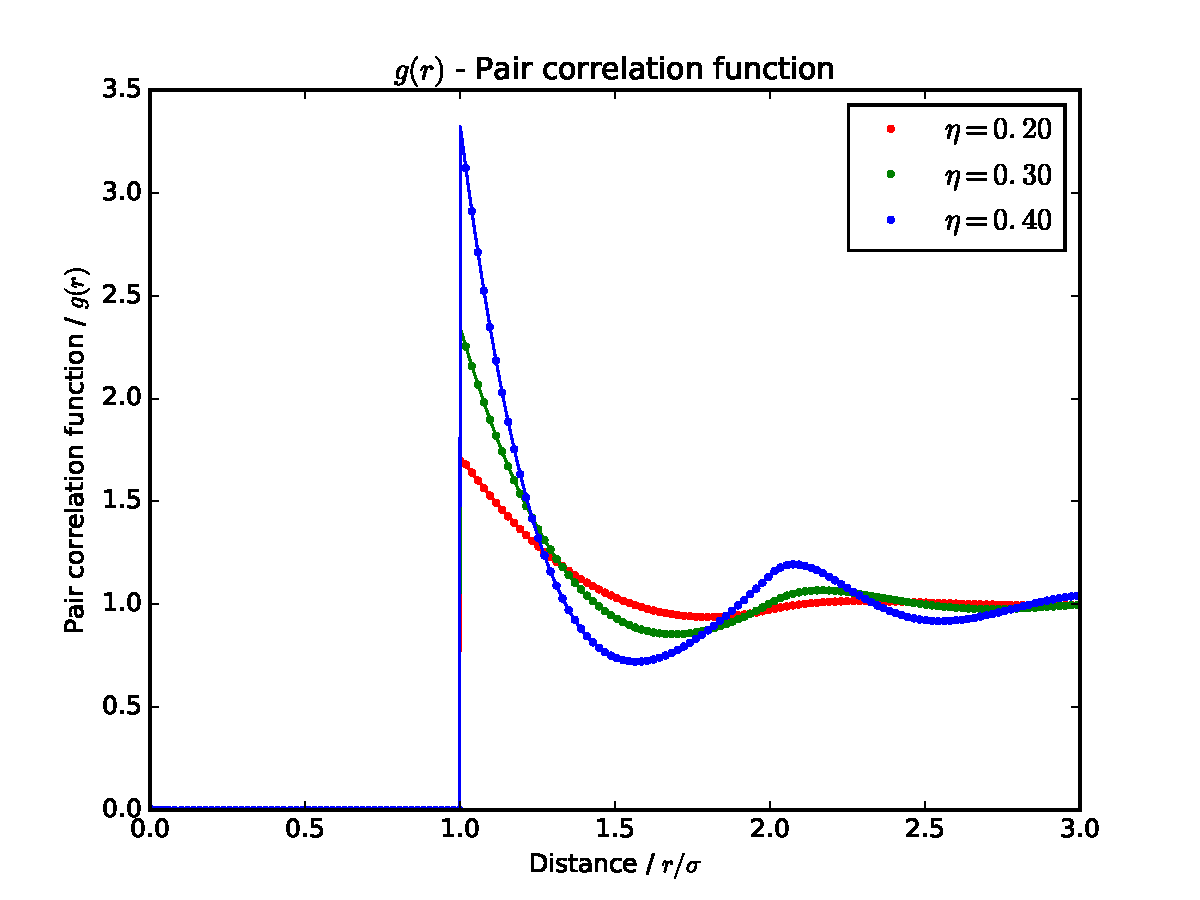
\includegraphics[width=0.7\textwidth]{{../graphs/ozsolver-g}.pdf}
  \end{center}
  \caption{Plot of the pair correlation function, $g(r)$, for several values of $\eta$. Points are values computed using the OZ solver, and lines are theoretical values.}
\end{figure}

\begin{figure}[H]
  \begin{center}
    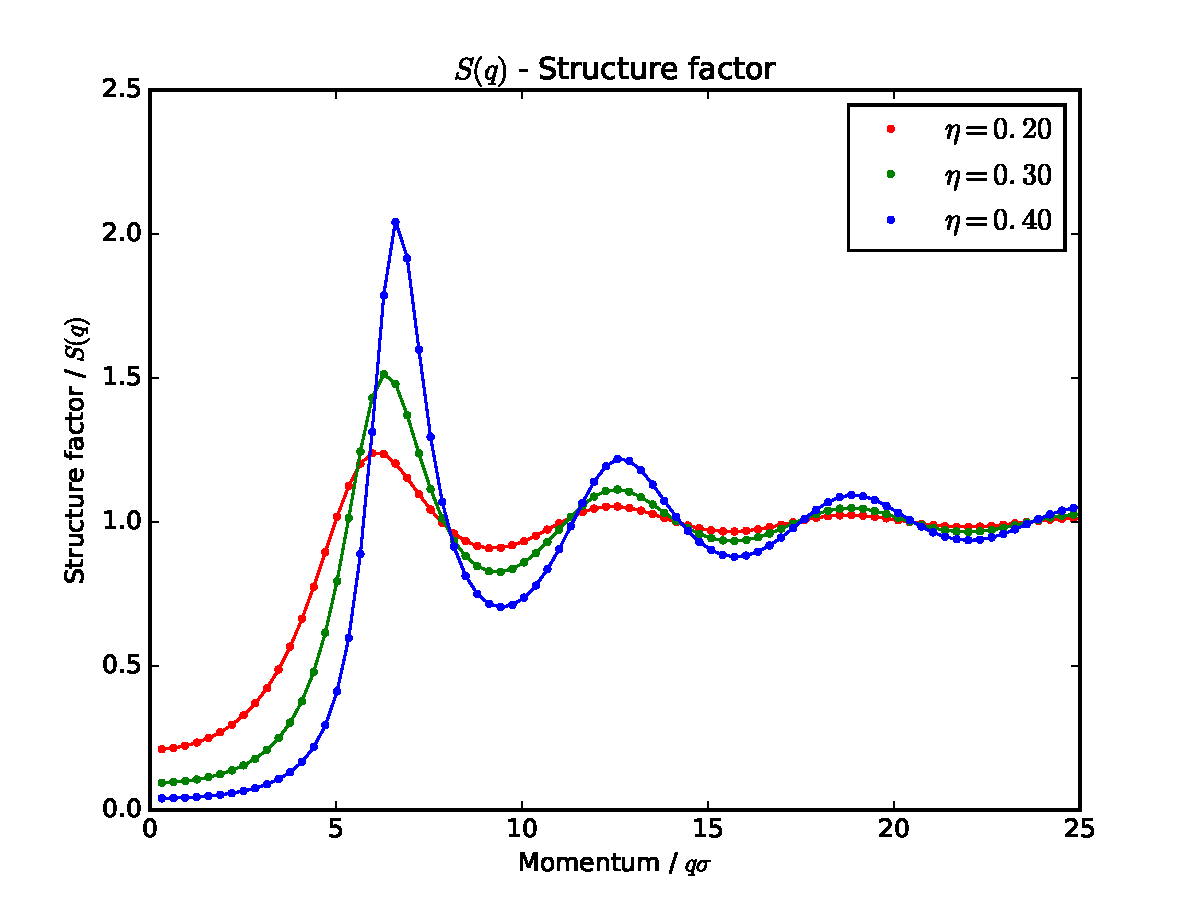
\includegraphics[width=0.7\textwidth]{{../graphs/ozsolver-s}.pdf}
  \end{center}
  \caption{Plot of the structure factor, $S(q)$, for several values of $\eta$. Points are values computed using the OZ solver, and lines are theoretical values.}
\end{figure}

We can notice the remarkable agreement between theoretical and numerical results, as we could have expected since the system we are considering, hard spheres, can be solved exactly without any approximations. As we could have expected, for values of $\eta$ closer to the freezing point $g(r)$ will take more negative values, since particles are more close together.

\end{document}
